\documentclass[conference,a4paper]{IEEEtran}
\IEEEoverridecommandlockouts
\usepackage{cite}               % sorts and compresses citations: [3]--[5], never [3][4][5]
\usepackage{amsmath,amssymb,amsfonts}
\usepackage{graphicx}
\usepackage{textcomp}
\usepackage{xcolor}
\usepackage{booktabs}
\usepackage{tikz}
\usetikzlibrary{arrows.meta, positioning, calc}
\usepackage[hidelinks]{hyperref}
\usepackage{times}
\sloppy

\setlength{\textfloatsep}{6pt plus 1pt minus 1pt}
\setlength{\floatsep}{4pt plus 1pt minus 1pt}
\setlength{\intextsep}{6pt plus 1pt minus 1pt}
\setlength{\abovecaptionskip}{3pt}
\setlength{\belowcaptionskip}{2pt}

% generated by scripts/make_thesis_tables.py -- do not edit
\newcommand{\nFullCorrect}{21}
\newcommand{\nFullWrong}{43}
\newcommand{\nFullAbstain}{35}
\newcommand{\nSPCorrect}{34}
\newcommand{\nSPWrong}{66}
\newcommand{\nTOCorrect}{15}
\newcommand{\nTOWrong}{51}
\newcommand{\nTOAbstain}{33}
\newcommand{\nGemCorrect}{30}
\newcommand{\nGemWrong}{51}
\newcommand{\nGemAbstain}{19}
\newcommand{\nStrictAbstain}{85}
\newcommand{\nFullPrec}{33}
\newcommand{\nSPPrec}{34}
\newcommand{\nGemPrec}{37}
\newcommand{\nDiffWrongSP}{22.7}
\newcommand{\nDiffCorrectSP}{12.7}
\newcommand{\nJudgeAgree}{22/25}
\newcommand{\nJudgeKappa}{0.72}
\newcommand{\nJudgeUnsure}{5}
\newcommand{\nSelFullHeld}{40}
\newcommand{\nSelFullAns}{31}
\newcommand{\nSelGemHeld}{14}
\newcommand{\nSelGemAns}{39}
\newcommand{\nProofOnRefFull}{31}
\newcommand{\nProofBoxesFull}{72}
\newcommand{\nProofInsideFull}{71}
\newcommand{\nCellsFull}{12/12}
\newcommand{\nCellsSP}{30/44}
\newcommand{\nCGSFull}{0.07}
\newcommand{\nPointFullAns}{0.28}
\newcommand{\nMultihopN}{10}
\newcommand{\nAnnotatedN}{50}
   % numbers quoted in the text, generated from the results

\begin{document}

\title{Gated and Grounded: An Agentic Multimodal RAG for Verifiable Question
Answering on Scientific Papers}

% --- Author block. Remove it for a double-blind submission; check the venue's rules. ---
%\author{
%\IEEEauthorblockN{Md Tamim Hossain\IEEEauthorrefmark{1} and Saad Al Abeed\IEEEauthorrefmark{2}}
%\IEEEauthorblockA{\IEEEauthorrefmark{1}\textit{Department of Computer Science and Engineering},
%\textit{Military Institute of Science and Technology (MIST)}, Dhaka, Bangladesh\\
%\IEEEauthorrefmark{2}\textit{Department of Computer Science and Engineering},
%\textit{Islamic University of Technology (IUT)}, Gazipur, Bangladesh\\
%Email: TODO, TODO}
%}

\maketitle

\begin{abstract}
Questions about scientific papers are often answered by tables and figures, yet
single-pass multimodal retrieval-augmented generation (RAG) answers every question,
supported or not, and gives the reader no way to check where a claim came from. In
this paper, an agentic multimodal RAG system is presented that gathers text, tables and
figures over several rounds, asks a sufficiency gate whether the gathered evidence is
enough before any answer is written, verifies each claim against the evidence it cites,
and draws a proof box on the page for every published claim. The system was built
with an open 4-bit 7B vision-language model on a single consumer GPU and evaluated on
150 questions from SPIQA against a single-pass and a text-only baseline. Answers were
graded by a model judge that agreed with a human grader on \nJudgeAgree{} answers
(kappa \nJudgeKappa). The agent was wrong on \nFullWrong\% of the questions, against
\nSPWrong\% for single-pass, but it was also correct less often (\nFullCorrect\% against
\nSPCorrect\%), because its abstentions did not fall on the harder questions. When the
same graph was run with a stronger model, abstention became selective. Where a claim
cited the correct table or figure, its proof box pointed at the hand-annotated answer
in \nProofInsideFull\% of cases, and every checked table-cell proof did. The gates are
therefore shown to cut confident errors, while their full benefit depends on the
capacity of the model that makes the judgements.
\end{abstract}

\begin{IEEEkeywords}
retrieval-augmented generation, multimodal question answering, agentic retrieval,
answer attribution, hallucination, scientific documents
\end{IEEEkeywords}

\section{Introduction}
\label{sec:intro}

A large share of what a scientific paper reports is never written out in its running
text. The decisive number sits in a table cell, and the trend that supports a claim is
drawn in a chart. A question answering system for papers therefore has to read tables
and figures, and benchmarks such as SPIQA~\cite{pramanick2024spiqa} were built for
exactly this setting: each question is tied to the figure or table that holds its
answer.

Most retrieval-augmented generation (RAG) systems~\cite{lewis2020rag} retrieve once and
then answer. When the retrieved material does not contain the answer, the generator
still produces one, and a fluent but unsupported answer is hard to tell apart from a
correct one. A second problem is verification. Even a correct answer is of limited use
to a researcher if the cell or chart region it rests on cannot be located, since the
answer then has to be checked by reading the paper anyway.

In this work, both problems are approached with the same idea: the system is made to
check before it answers. An agent gathers evidence over several rounds, choosing the
next tool from a text, a table and a figure retriever. A sufficiency gate decides
whether the evidence suffices before anything is written. Each claim of the draft must
cite its evidence, and a faithfulness gate verifies every citation. Every published
claim is then grounded by a box on the page: a table cell, a chart bar, a quoted
sentence or a diagram label. When the evidence does not suffice, the system says so
instead of guessing.

Three research questions were studied:
\begin{itemize}
    \item \textbf{RQ1:} Does the agentic loop with its gates improve accuracy and reduce
    wrong answers compared with single-pass retrieval?
    \item \textbf{RQ2:} Can visual document retrieval bring the right tables and figures
    to the agent, and does seeing them help?
    \item \textbf{RQ3:} Can the agent ground its claims with precise boxes on the page?
\end{itemize}

The main contributions are as follows:
\begin{itemize}
    \item An agentic multimodal RAG design with two gates and verified claim
    citations, implemented end to end with an open model on consumer hardware.
    \item An exact grounding scheme that boxes cells, bars, sentences and labels read
    from the PDF, with the retriever's similarity map kept only for photographs.
    \item A three-way evaluation (correct, wrong, abstained) with a checked model judge,
    an analysis of whether abstention is selective, and hand-annotated answer regions.
    \item Evidence, obtained by keeping the graph fixed and changing only the model,
    that the benefit of the gates is bounded by the model that makes their judgements.
\end{itemize}

The rest of the paper is organised as follows. Related work is reviewed in
Section~\ref{sec:related}, and the system is described in Section~\ref{sec:method}. The
experimental setup is given in Section~\ref{sec:setup}, the results are reported in
Section~\ref{sec:results}, and they are discussed in Section~\ref{sec:discussion}.
Section~\ref{sec:conclusion} concludes the paper.

\section{Related Work}
\label{sec:related}

\subsection{Question Answering over Document Images}

Questions about the visual content of documents were made a benchmark task by
DocVQA~\cite{mathew2021docvqa}, and ChartQA~\cite{masry2022chartqa} added questions that
require values and trends to be read from charts. SPIQA~\cite{pramanick2024spiqa}
carries the task to scientific papers and annotates the reference figure or table of
each question. These benchmarks score whether an answer is correct; the location of
its evidence is not asked for, which leaves the verification problem open.

\subsection{Visual Document Retrieval}

Late interaction, introduced for passages by ColBERT~\cite{khattab2020colbert}, scores
a query by matching each of its tokens to the most similar document token.
ColPali~\cite{faysse2025colpali} applies the same scoring to page images embedded as
grids of patches, so that pages can be retrieved without OCR. On top of such
retrievers, VisRAG~\cite{yu2024visrag} and M3DocRAG~\cite{cho2024m3docrag} pass the
retrieved page images to a vision-language generator. In both systems retrieval is
performed once, whereas in the present system pages and regions are retrieved
repeatedly under the control of a planner.

\subsection{Agentic and Self-Correcting RAG}

In ReAct~\cite{yao2023react}, reasoning steps and tool calls are interleaved, so that
each observation shapes the next action. Self-RAG~\cite{asai2024selfrag} trains a model
to decide when to retrieve and to critique its own output, and Corrective
RAG~\cite{yan2024crag} grades the retrieved documents and retrieves again when they are
poor. The two gates used here play comparable roles, but they are realised by
prompting an off-the-shelf model without training, and they judge evidence from three
modalities. Abstention has been studied as selective question
answering~\cite{kamath2020selective}; the same question, whether a system abstains on
the right inputs, is asked here of the agent.

\subsection{Attribution and Evaluation}

ALCE~\cite{gao2023alce} measures how well generated statements are supported by the
passages they cite. RAGAS~\cite{es2024ragas} uses a language model as the evaluator of
RAG answers, and the reliability of such judges has been examined
directly~\cite{zheng2023judge}. For visual attribution, the pointing
game~\cite{zhang2018pointing} tests whether the peak of a saliency map falls on the
annotated object; the same test is applied in this work to proof boxes.

\section{Proposed System}
\label{sec:method}

\subsection{Overview}

The system is built as a graph of nodes, each with a single task, in
LangGraph~\cite{langgraph}. The flow of a question through the graph is shown in
Fig.~\ref{fig:pipeline}. The question is first analysed; the planner then selects one
retrieval tool per round, and the results are added to an evidence buffer. The
sufficiency gate (G1) either sends control back to the planner for another round or
releases the buffer to the writer. The writer drafts claims with citations, the
faithfulness gate (G2) checks every claim and returns failed drafts for rewriting, and
the accepted claims are grounded with proof boxes before the answer is returned. Two
loops are therefore present, and both are bounded: at most three retrieval rounds and
at most two rewrites are allowed.

\begin{figure}[!htb]
\centering
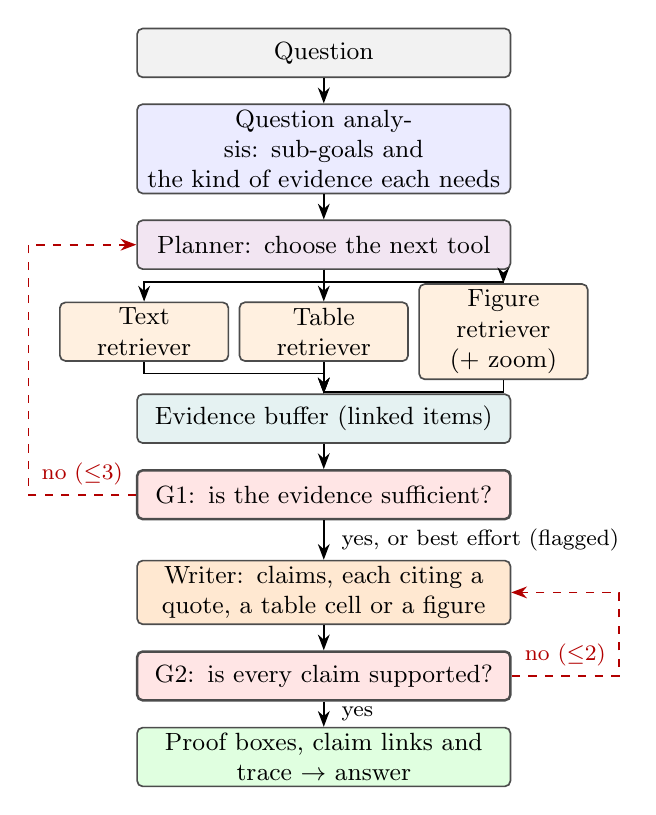
\begin{tikzpicture}[
  font=\small,
  node distance=3.2mm,
  box/.style={draw=black!70, rounded corners=2pt, line width=0.6pt, align=center,
              text width=4.6cm, minimum height=6.2mm, inner sep=2pt, fill=#1},
  box/.default=white,
  tool/.style={draw=black!70, rounded corners=2pt, line width=0.6pt, align=center,
               text width=2.0cm, minimum height=6.2mm, inner sep=2pt, fill=orange!12},
  gate/.style={box=red!10, line width=0.9pt},
  arr/.style={-{Stealth[length=2mm]}, line width=0.6pt},
  back/.style={-{Stealth[length=2mm]}, line width=0.6pt, dashed, red!70!black},
  lab/.style={font=\footnotesize, align=left}
]
\node[box=gray!10] (q) {Question};
\node[box=blue!8, below=of q] (ana) {Question analysis: sub-goals and\\ the kind of evidence each needs};
\node[box=violet!10, below=of ana] (plan) {Planner: choose the next tool};
\node[tool, below=4mm of plan] (tab) {Table\\ retriever};
\node[tool, left=1.2mm of tab] (txt) {Text\\ retriever};
\node[tool, right=1.2mm of tab] (fig) {Figure\\ retriever (+ zoom)};
\node[box=teal!10, below=4mm of tab] (buf) {Evidence buffer (linked items)};
\node[gate, below=of buf] (g1) {G1: is the evidence sufficient?};
\node[box=orange!18, below=5mm of g1] (wr) {Writer: claims, each citing a\\ quote, a table cell or a figure};
\node[gate, below=of wr] (g2) {G2: is every claim supported?};
\node[box=green!12, below=of g2] (out) {Proof boxes, claim links and\\ trace $\rightarrow$ answer};

\draw[arr] (q) -- (ana);
\draw[arr] (ana) -- (plan);
\draw[arr] (plan) -- (tab);
\draw[arr] (plan.south) -- ++(0,-1.5mm) -| (txt.north);
\draw[arr] (plan.south) -- ++(0,-1.5mm) -| (fig.north);
\draw[arr] (tab) -- (buf);
\draw[arr] (txt.south) -- ++(0,-1.5mm) -| (buf.north);
\draw[arr] (fig.south) -- ++(0,-1.5mm) -| (buf.north);
\draw[arr] (buf) -- (g1);
\draw[arr] (g1) -- node[lab, right=1mm] {yes, or best effort (flagged)} (wr);
\draw[arr] (wr) -- (g2);
\draw[arr] (g2) -- node[lab, right=1mm] {yes} (out);
% the two loops run outside the row of tools, with their labels on the horizontal segment
\coordinate (xl) at (-3.75,0);
\coordinate (xr) at (3.75,0);
\draw[back] (g1.west) -- node[lab, above, midway] {no ($\leq$3)} (g1.west -| xl) |- (plan.west);
\draw[back] (g2.east) -- node[lab, above, midway] {no ($\leq$2)} (g2.east -| xr) |- (wr.east);
\end{tikzpicture}
\caption{Flow of a question through the system. Solid arrows show the forward path.
Dashed arrows show the two bounded loops: the sufficiency gate (G1) returns control to
the planner for another round (at most three), and the faithfulness gate (G2) returns
the draft to the writer (at most two rewrites).}
\label{fig:pipeline}
\end{figure}

\subsection{Question Analysis and Planning}

The question is split into sub-goals, and the names it mentions (datasets, methods,
metrics) are extracted for later filtering. The kind of evidence each sub-goal needs,
a table or a figure, is not left to the language model. It is decided by a vote of the
nine most similar labelled SPIQA questions taken from papers that are used in neither
the development nor the test split. On the development questions, this vote chose the
reference's kind in 17 of 20 cases, whereas the model alone chose it in 8. The planner
then selects one tool per round and writes the query for it; a tool that has already
been used for a sub-goal may be called again only with a new query.

\subsection{Retrieval Tools}

Three tools can be selected by the planner. The text retriever ranks the paper's
paragraphs by reciprocal rank fusion~\cite{cormack2009rrf} of two lists: SPECTER2
embeddings~\cite{singh2023scirepeval} searched with FAISS~\cite{johnson2019faiss}, and
keyword overlap weighted by inverse document frequency. The keyword list was added
because, within one paper, every paragraph shares the topic that the embedding
captures, whereas SPIQA questions reuse the paper's own terms. The table retriever
ranks the paper's tables by their caption words and by the visual score of their page,
and returns each table as cells recovered with Table Transformer~\cite{smock2022pubtables},
each cell keeping its page coordinates. The figure retriever scores page images with
ColQwen2, a model of the ColPali family~\cite{faysse2025colpali}, and returns the best
figure. A fourth tool, a zoom that re-renders the figure at 300~dpi, is not chosen by
the planner; it is run automatically when a figure covers less than 30\% of its page.
Every retrieved item enters the evidence buffer with its page, tool and round, and
items are linked when they share a page or when a sentence names a table or figure.

\subsection{Sufficiency Gate}

Before anything is written, the buffer is judged by G1. The gate is asked to name the
facts in the buffer that answer the question, with their evidence identifiers, and to
give its verdict only afterwards. The order matters because the reply is generated as
JSON in schema order: when the verdict came first, it was justified only after it had
been made. If G1 is not convinced after three rounds, two cases are separated. When no
answering fact was found, the system abstains and reports what is missing. When such
facts were found but judged incomplete, the answer is written from them as a
\emph{best effort} and is marked as possibly incomplete. In this way, G1 decides when
the search stops, while the decision to publish a claim is left to G2.

\subsection{Writing and Faithfulness Gate}

The writer receives the buffer as text, cells and figure images, and returns a list of
claims. Every claim must cite its evidence as a verbatim quote, a table cell given by
row, column and value, or an observation about a figure. Each citation is verified by
G2 in two layers. First, a quote must occur in the cited paragraph and a cell value
must equal the parsed cell; both sides are normalised beforehand for the artefacts of
PDF text extraction, such as ligatures, line-end hyphens and spaced decimals. Second,
the model is asked whether the cited evidence supports the claim as written. A failed
draft is returned with the reason, and claims that still fail after two rewrites are
withheld and listed as unconfirmed.

\subsection{Grounding the Claims}

Every published claim is given a box on the page, and exact sources are preferred: the
cited table cell, the bar of a vector chart read directly from the PDF, the quoted
sentence located on the page, the caption, or the labels of a diagram that the claim
names. Only for photographs, which carry no printed words, is the box taken from the
highest-scoring patches of the ColQwen2 similarity map computed for the claim's text.
An execution trace, listing the tools called and every gate decision, is returned with
the answer.

\section{Experimental Setup}
\label{sec:setup}

\subsection{Data}

Questions were drawn from SPIQA test-A~\cite{pramanick2024spiqa} (118 papers, 666
questions) with a fixed seed. Whole papers were assigned to the splits, so that no
paper contributes to both. A development split of 20 questions from 5 papers was used
for every design decision. A test split of 150 questions from 31 papers (71 with a
table and 79 with a figure as reference, at most 8 per paper) was used once. All
settings were frozen before the test run, and the evaluation script refuses to run on
the test split if any setting differs. A multi-hop subset of \nMultihopN{} test
questions was selected by a fixed rule over the question text: it holds the questions
that ask for a reason or an implication (``why'', ``suggest'', ``possible
explanation'') of a result shown in a table or figure.

\subsection{Systems Compared}

The same model, tools, prompts and grounding are used by every system, and each system
removes one part of the design. \emph{Full} is the complete agent. \emph{Single-pass}
has no planner, loops or gates: every tool is called once with the question, and the
writer answers from the result, so that the effect of agency is isolated.
\emph{Text-only} is the full graph with the text tool alone, with tables and figures
available only as extracted text, so that the effect of seeing them is isolated.
\emph{Strict G1} is the first frozen design, in which the agent abstains whenever G1
is not convinced (Section~\ref{sec:best-effort}). \emph{Full (Gemini)} is the full graph
with Gemini~3.5 Flash-Lite (free tier) behind every model call, so that the effect of
the model is separated from that of the architecture.

\subsection{Implementation}

The language model is Qwen2.5-VL-7B-Instruct~\cite{bai2025qwen25vl}, quantised to
4~bits and served by llama.cpp. All experiments were run offline on one
PC with an Intel Arc B580 GPU (12~GB) and 15.6~GB of RAM. Every model reply is
constrained to a JSON schema, generated at temperature 0 with a fixed seed, and cached
under a hash of the request, so that every answer can be reproduced exactly.

\subsection{Outcomes and Judge}

One of three outcomes is assigned to each question. It is \emph{correct} or
\emph{wrong} when at least one claim reaches the reader, and \emph{abstained} when the
system reports that it could not confirm an answer or when every claim is withheld by
G2. Answers were graded against SPIQA's gold answer by the local model, which was told
to accept an answer that gives the main point of the gold answer and contradicts
nothing in it, and to write its reason before its verdict. To check the judge, 30
answers (6 per system, shuffled) were graded by a human annotator who did not know the
system or the judge's verdict.

\subsection{Metrics}

Besides the outcome rates and the precision when answering, four scores were computed.
Retrieval faithfulness (RF) is the share of the distinct tables and figures in the
buffer that are the reference, and the hit rate is the share of questions whose
reference reached the buffer. The agent efficiency score (AES) is the number of hops
needed (one, or two on the multi-hop subset) divided by the number of search calls,
capped at one. The cross-modal grounding score (CGS) is the best intersection over union
(IoU) between a proof box and a hand-drawn answer box, with zero for a question
without a box. Since IoU was found to penalise correct proofs drawn at another size
(Section~\ref{sec:rq3}), the pointing game~\cite{zhang2018pointing} is also reported: a
proof counts as a hit when the centre of its box lies inside an answer box. This measure
was added after the IoU results were seen. Finally, the share of published claims that
cite the reference table or figure is reported as reference attribution. All rates are
given with 95\% bootstrap intervals over questions (10{,}000
resamples), and differences are paired by question.

\subsection{Annotation}

For the grounding scores, 50 test questions (25 tables and 25 figures) were drawn at
random before any output was inspected. On each page, the part of the table or figure
holding the gold answer was boxed by a co-author with an offline annotation tool and
written guidelines. In two quality-control rounds, 16 boxes that covered a whole table
or figure although the question named specific values were narrowed; they were
selected by a fixed rule, without reference to any system's boxes.

\section{Results}
\label{sec:results}

\subsection{Overall Outcomes}

The outcomes of the five systems on the 150 test questions are given in
Table~\ref{tab:outcomes}, together with the precision when answering, that is, the
share of answered questions that were answered correctly. The full agent answered
\nFullCorrect\% of the questions correctly, was wrong on \nFullWrong\% and abstained on
\nFullAbstain\%. Single-pass, which never abstains, was correct on \nSPCorrect\% and
wrong on \nSPWrong\%.

\begin{table}[!htb]
\centering
\caption{Outcomes on the 150 test questions in percent, with 95\% bootstrap intervals
in brackets, and precision when answering (Prec.)}
\label{tab:outcomes}
\footnotesize
% generated by scripts/make_conference_tables.py -- do not edit
\setlength{\tabcolsep}{3.5pt}
\begin{tabular}{lcccc}
\toprule
System & Correct & Wrong & Abstained & Prec. \\
\midrule
Full (7B) & 21 [15, 28] & 43 [35, 51] & 35 [28, 43] & 33 \\
Single-pass & 34 [27, 41] & 66 [59, 73] & 0 [0, 0] & 34 \\
Text-only & 15 [10, 21] & 51 [43, 59] & 33 [26, 41] & 23 \\
Strict G1 & 5 [2, 9] & 9 [5, 14] & 85 [79, 91] & 36 \\
Full (Gemini) & 30 [23, 37] & 51 [43, 59] & 19 [13, 26] & 37 \\
\bottomrule
\end{tabular}

\end{table}

The same outcomes are drawn in Fig.~\ref{fig:outcomes}, where the trade made by each
system can be seen directly: the gated systems replace part of the wrong answers with
abstentions, and the strict design replaces most answers of every kind.

\begin{figure}[!htb]
\centering
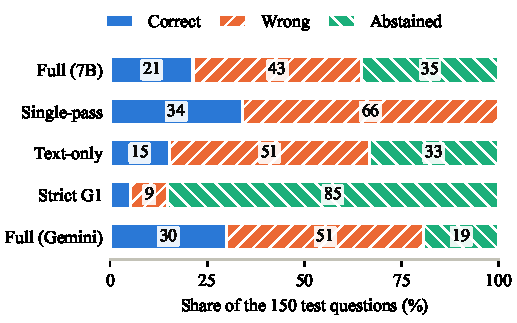
\includegraphics[width=\columnwidth]{figures/fig_outcomes.pdf}
\caption{Share of correct, wrong and abstained answers for each system on the 150 test
questions. Hatching distinguishes the outcomes in grey-scale print.}
\label{fig:outcomes}
\end{figure}

The judge was found to be reliable. It agreed with the human grader on \nJudgeAgree{}
answers (Cohen's kappa of \nJudgeKappa), and \nJudgeUnsure{}
further answers were left undecided by the grader. In all three disagreements, the
answer was accepted by the human and rejected by the judge, so the correct rates in
Table~\ref{tab:outcomes} are, if anything, conservative.

\subsection{RQ1: Agency}

The paired differences between the systems are listed in Table~\ref{tab:differences}.
Compared with single-pass, the full agent was wrong \nDiffWrongSP{} percentage points
less often, and the difference lies outside the bootstrap interval. It was also
correct \nDiffCorrectSP{} points less often, because \nFullAbstain\% of the questions
were left unanswered. Its precision when answering (\nFullPrec\%) was no higher than
that of single-pass (\nSPPrec\%), which shows that fewer wrong answers were obtained by
answering less rather than by answering better.

\begin{table}[!htb]
\centering
\caption{Paired differences in percentage points on the same questions
($^{*}$: the 95\% bootstrap interval excludes zero; MH: multi-hop subset)}
\label{tab:differences}
\footnotesize
% generated by scripts/make_conference_tables.py -- do not edit
\begin{tabular}{lccc}
\toprule
Comparison & Correct & Wrong & Abstained \\
\midrule
Full $-$ Single-pass & $-12.7$$^{*}$ & $-22.7$$^{*}$ & $+35.3$$^{*}$ \\
Full $-$ Text-only & $+6.0$ & $-8.0$ & $+2.0$ \\
Full $-$ Strict G1 & $+16.0$$^{*}$ & $+34.0$$^{*}$ & $-50.0$$^{*}$ \\
Gemini $-$ Full (7B) & $+8.7$ & $+7.3$ & $-16.0$$^{*}$ \\
\midrule
Full $-$ Single-pass, MH & $+20.0$ & $-40.0$$^{*}$ & $+20.0$ \\
Full $-$ Text-only, MH & $+40.0$$^{*}$ & $+0.0$ & $-40.0$$^{*}$ \\
\bottomrule
\end{tabular}

\end{table}

Whether the abstentions fall on the hard questions was tested with single-pass as a
reference. A selective agent would hold back the questions that single-pass also gets
wrong. The opposite was observed: single-pass was correct on \nSelFullHeld\% of the
questions that the full agent held back, but on only \nSelFullAns\% of those it answered.
The best-effort flag carried little information as well, since flagged answers were
correct about as often as those accepted by G1 (24 of 75 against 8 of 22). On the
multi-hop subset, where the loop was expected to matter most, the full agent was wrong
on 2 of the 10 questions against 6 for single-pass, but ten questions allow only an
indicative reading. The search tools were called 2.7 times per question by the agent and
3 times by single-pass, which gives a higher efficiency score (AES 0.44 against 0.36).
The planner and the gates, however, raised the number of model calls from 3 to 11.7
per question.

\subsection{A Change Made During Evaluation}
\label{sec:best-effort}

In its first frozen form, the agent abstained whenever G1 was not convinced after three
rounds. In the first test run, 110 of the first 142 questions were abstained before a
power cut stopped the run, although the reference was in the buffer for about two
thirds of them. The best-effort rule of Section~\ref{sec:method} was then designed on
the development split only, without any test answer being read; on that split it
moved the agent from 6 right, 1 partly right, 0 wrong and 13 abstained to 9, 4, 5 and
2. All systems were re-run on the test split, and the first design was kept as the
strict G1 ablation.

\subsection{RQ2: Visual Retrieval}

The reference table or figure reached the buffer for 73\% of the questions with the
full agent and for 77\% with single-pass, which fetches every kind of evidence in every
run. Of the distinct tables and figures fetched by the agent, 44\% were the reference
(RF 0.44, against 0.41 for single-pass and 0.55 with Gemini). On the development
split, ColQwen2 ranked the reference's page first for 15 of 20 questions. Compared with the text-only agent, the full agent was correct 6 points more
often and wrong 8 points less often (Table~\ref{tab:differences}), and neither
difference lies outside its interval. On the multi-hop subset, however, the full agent
was correct 40 points more often.

\subsection{RQ3: Grounding}
\label{sec:rq3}

The grounding scores on the 50 annotated questions are given in
Table~\ref{tab:grounding}. Measured by IoU, grounding was poor for every system. On
inspection, a correct proof was often scored low because it was drawn at a different
size: a parsed cell spans the width of its column, while the hand box was drawn
tightly around the printed number, so that two exactly right cells scored IoU 0.43 and
0.46. Shrinking each cited cell to its printed words did not raise CGS (0.070 against
0.068), as many questions lost as gained. The pointing game removes this effect, and it
credits the full agent on \nPointFullAns{} of its answered questions.

\begin{table}[!htb]
\centering
\caption{Grounding on the 50 annotated questions (CGS: best IoU; Point.: pointing game,
all and answered questions) and reference attribution on all 150 questions}
\label{tab:grounding}
\footnotesize
% generated by scripts/make_conference_tables.py -- do not edit
\begin{tabular}{lcccc}
\toprule
System & CGS & Point. & Point.\ (ans.) & Ref.\ attr. \\
\midrule
Full (7B) & 0.07 & 0.16 & 0.28 & 0.44 \\
Single-pass & 0.15 & 0.40 & 0.40 & 0.42 \\
Text-only & 0.00 & 0.04 & 0.07 & 0.00 \\
Full (Gemini) & 0.05 & 0.20 & 0.26 & 0.55 \\
\bottomrule
\end{tabular}

\end{table}

The low scores were traced to the choice of sources rather than to the boxes. Of the
\nProofBoxesFull{} proof boxes drawn by the full agent on the annotated questions, only
\nProofOnRefFull{} lay on the reference table or figure; the others pointed at
paragraphs or at other tables. Of the boxes on the reference, \nProofInsideFull\% pointed
inside the hand-drawn answer box, and every table-cell proof did (\nCellsFull). For
single-pass, whose cells are not checked by a gate, \nCellsSP{} cell proofs were inside.

\subsection{A Stronger Model behind the Same Graph}

With Gemini behind every call and nothing else changed, the agent was correct on
\nGemCorrect\%, wrong on \nGemWrong\% and abstained on \nGemAbstain\%. G1 was convinced on
117 questions instead of 22, after 1.9 rounds on average instead of 2.7, and G2 kept
88\% of the drafted claims instead of 50\%. Most importantly, its abstention was
selective: single-pass was correct on only \nSelGemHeld\% of the questions it held back,
against \nSelGemAns\% of those it answered.

\section{Discussion}
\label{sec:discussion}

\subsection{The Model Limits the Gates}

The design rests on the expectation that a system which checks its evidence and its
claims would turn confident errors into stated gaps. With the 7B model, only half of
this expectation was met: wrong answers became far less frequent, but easy questions
were held back as readily as hard ones. Because the graph, prompts and settings were
kept identical when the model was exchanged, the two explanations can be separated.
With the stronger model, G1 was convinced about five times as often, far fewer claims
were rejected by G2, and the held-back questions were the hard ones. The gates
therefore behave as intended when the model behind them can judge sufficiency and read
tables and charts reliably, and a 4-bit 7B model cannot yet do so consistently. A
practical arrangement follows from this result: a small local model can read and
write, while the two judgements are delegated to a stronger model.

\subsection{Measuring Grounding}

IoU against a hand-drawn box was fixed as the grounding measure before the evaluation,
but it was found to compare two drawing conventions as much as the precision of a
proof. A cell box spans its column, while an annotator boxes the number, or a whole
row for a comparison. The pointing game is insensitive to these conventions and is
therefore reported next to IoU. In future annotation, the unit should be fixed in
advance, for instance whole cells for tables.

\subsection{Threats to Validity}

The judge is the same model as the evaluated local systems; its agreement with a human
grader was substantial, but it was checked on 25 answers only. The answer boxes were
drawn by one annotator who, as a co-author, knew the aims of the work. The best-effort
rule was introduced after a first test run, and the pointing game after the IoU
results; both are disclosed, and the original measures are reported. The study covers
150 questions from 31 computer-science papers, retrieval within a known paper, one
quantised model run once at temperature 0, and a multi-hop subset of ten questions.
Reference attribution, used in place of a hand check of each citation, undercounts
claims that correctly cite supporting text. Finally, the benefit of proof boxes for
human verification was argued from their precision and was not measured in a user
study.

\section{Conclusion}
\label{sec:conclusion}

An agentic multimodal RAG system was presented that gathers evidence over several
rounds, checks the sufficiency of the evidence before writing, verifies every claim
against its citation, and grounds each published claim with a box on the page. On 150
SPIQA questions, wrong answers were reduced from \nSPWrong\% to \nFullWrong\% compared
with single-pass retrieval, at the cost of abstentions that, with a 7B model, did not
single out the hard questions; with a stronger model behind the same graph, abstention
became selective. Where a claim cited the right table or figure, its proof box pointed
at the answer in \nProofInsideFull\% of cases. In future work, a hybrid in which a small
model reads and writes while a stronger model makes the two judgements will be
evaluated on unused SPIQA papers, claims will be steered towards the table or figure
that holds the answer, and the value of the proofs for human verification will be
measured in a user study.


\bibliographystyle{IEEEtran_doi}  % IEEEtran.bst + the doi field (IEEE style requires DOIs)
\bibliography{references}

\end{document}
